%\documentclass{uai2021} % for initial submission
 \documentclass[accepted]{uai2021} % after acceptance, for a revised
                                    % version; also before submission to
                                    % see how the non-anonymous paper
                                    % would look like
% NOTE: Only comment/uncomment the lines above as appropriate,
%       as they will be replaced automatically for papers to be published.
%       Do not make any other change above this note for an accepted
%       version.

%% Choose your variant of English; be consistent
\usepackage[american]{babel}
% \usepackage[british]{babel}

%% Some suggested packages, as needed:
\usepackage{natbib} % has a nice set of citation styles and commands
    \bibliographystyle{plainnat}
    \renewcommand{\bibsection}{\subsubsection*{References}}
\usepackage{mathtools} % amsmath with fixes and additions
% \usepackage{siunitx} % for proper typesetting of numbers and units
\usepackage{booktabs} % commands to create good-looking tables
\usepackage{tikz} % nice language for creating drawings and diagrams

%%%%%%%%%%%%%%%%%%%%%%%%%%%

\usepackage{amsfonts}
\usepackage{amsthm}
\usepackage{comment}
\usepackage{dsfont}

%%%%%%%%%%%%%%%%%%%%%%%%%%%

%% Provided macros
% \smaller: Because the class footnote size is essentially LaTeX's \small,
%           redefining \footnotesize, we provide the original \footnotesize
%           using this macro.
%           (Use only sparingly, e.g., in drawings, as it is quite small.)

%% Self-defined macros
\newcommand{\md}{\mathrm{d}}

%%%%%%%%%%%%%%%%%%%%%%%%%%%

\newtheorem{thm}{Theorem}
\newtheorem{algo}[thm]{Algorithm}
\newtheorem{ass}[thm]{Assumption}
\newtheorem{cor}[thm]{Corollary}
\newtheorem{defn}[thm]{Definition}
\newtheorem{exmp}[thm]{Example}
\newtheorem{lem}[thm]{Lemma}
\newtheorem{prop}[thm]{Proposition}
\newtheorem{rem}[thm]{Remark}


\newcommand{\pa}{\textnormal{pa}}

\newcommand{\ds}{\text{ds}}
\newcommand{\dt}{\text{dt}}

\newcommand{\disjU}{\mathbin{\dot{\cup}}}

\newcommand{\norm}[1]{\left\lVert#1\right\rVert}

\usepackage{tikz}
\usepgflibrary{arrows}
\usetikzlibrary{shapes}
\usetikzlibrary{arrows.meta}
\usetikzlibrary{positioning}

\usepackage{graphicx}
\usepackage{caption}
\usepackage{subcaption}


%%%%%%%%%%%%%%%%%%%%%%%%%%%


\title{Equality Constraints in Linear Hawkes 
Processes}

% The standard author block has changed for UAI 2021 to provide
% more space for long author lists and allow for complex affiliations
%
% All author information is authomatically removed by the class for the
% anonymous submission version of your paper, so you can already add your
% information below.
%
% Add authors in order of decreasing contribution
\author[1]{\href{mailto: Søren Wengel Mogensen 
<soren.wengel_mogensen@control.lth.se>}{Søren~Wengel~Mogensen}{}} 
% Add affiliations after the authors
\affil[1]{%
    Department of Automatic Control\\
    Lund University\\
    Sweden
}

\begin{document}
\maketitle

\begin{abstract}
Conditional independence is often used as a testable 
implication of causal models of random variables. In addition, equality 
constraints have been proposed to distinguish between data-generating 
mechanisms. We show that one 
can also find equality constraints in linear Hawkes processes, 
extending this theory to a class of continuous-time stochastic processes. This 
is done by proving that Hawkes process models in a certain sense satisfy the 
equality 
constraints 
of linear structural equation models. These results
allow more refined constraint-based structure learning in this class of 
processes. Arguing for the existence of equality constraints leads us to 
new 
identification 
results for Hawkes processes. We also describe a causal interpretation of the 
linear 
Hawkes process which is closely 
related to its so-called cluster representation.

\end{abstract}


\section{Introduction}\label{sec:intro}

In causal inference, the question of what can be learnt about the underlying 
structure from observational data is a classical one 
\citep{spirtes1993,pearl2009}. While most work 
studies models of random variables and without an explicit notion of time, this 
question has also been 
studied for stochastic process models. For a multivariate stochastic 
process, $X_t = (X_t^1, X_t^2, \ldots, X_t^n)^T$, this is often formalized by 
assuming that the dynamical evolution of each coordinate process, $X_t^i$,   
depends directly only on a subset of the other coordinate processes which can 
be 
represented by a directed graph which is the \emph{structure} that methods 
aim to learn. As examples of this, \cite{eichlerHawkes2017, xu2016} learn
graphs describing the structure of multivariate linear Hawkes processes from 
dynamical observation of the process whereas 
\cite{achab2017} use integrated cumulants of 
linear Hawkes processes for structure learning. 
These approaches assume that we have full observation in the sense that every 
coordinate 
process is observed. \cite{meek2014, mogensenUAI2018, mogensenUAI2020} consider 
structure learning based on tests of so-called local independence and provide 
methods 
that can recover structural information based on a marginal distribution only. 

In this paper, we show that one can 
use equality 
constraints in linear Hawkes processes to distinguish between graphical 
structures that 
are indistinguishable using tests of local independence only which enables more 
refined structure learning algorithms. This development parallels that of 
structural causal models without an explicit notion of 
time in which equality constraints have 
been used for structure learning in addition to conditional independence 
constraints 
\citep{robins1986,vermaEquiAndSynthesis,robins1999,tian2002,shpitser2014,richardson2017}.


%%%%%%%%%%%%%%%%%%%%%%%%%%%
%%%%%%%%%%%%%%%%%%%%%%%%%%%

\section{Hawkes Processes}
\label{sec:hawPro}

Hawkes processes have received much attention in machine learning in recent 
years as a tractable model of mutually exciting streams of events 
\citep{zhou2013b,luo2015,etesami2016,tan2018,xu2018,trouleau2019}. 
The following is a brief introduction to this model class,
see \cite{laubHawkes2015}, \cite{linigerThesis}, and \cite{daleyVere} for 
additional background on Hawkes processes and point processes in general.

We consider a filtered probability space $(\Omega, \mathcal{F}, 
(\mathcal{F}_t), P)$ and an $n$-dimensional point process, $X_t = 
(X_t^1,X_t^2,\ldots,X_t^n)^T$, and let $V= \{1,2\ldots, n\}$. $\mathcal{F}_t$ 
is 
a filtration, that is, a nondecreasing family of $\sigma$-algebras which for 
each time point, $t\in \mathbb{R}$, represent the available information at 
that time. For each 
$\alpha\in 
V$, we say that $X^\alpha$ is a \emph{coordinate process}. Each coordinate 
process is described by a series of \emph{events}, or \emph{points}, that occur 
at time points indexed by $\mathbb{R}$. For $\alpha \in V$, this is formalized 
by random variables, $\{T_i^\alpha\}_{i\in\mathbb{Z}}$, such 
that $T_i^\alpha < T_{i+1}^\alpha$ almost surely. For $s<t$, we let the  
$N_t^\alpha - 
N_s^\alpha$ denote the number of points (events) in the $\alpha$-process 
in the interval $(s,t]$, that is,  $N_t^\alpha - 
N_s^\alpha= \sum_i \mathds{1}_{s < T_i^\alpha \leq t}$. We 
assume that no 
two events occur simultaneously. For 
$\alpha\in V$ the \emph{intensity process}, $\lambda_t^\alpha$, 
satisfies

$$
\lambda_t^{\alpha} = \lim_{h \downarrow 0} \dfrac{1}{h} P(N_{t + h}^\alpha  - 
N_t^\alpha = 1
\mid \mathcal{F}_t).
$$

The intensity, $\lambda^\alpha$, therefore describes how likely an 
$\alpha$-event is in the immediate future $(t, t+h]$, for small $h$, given the 
past until time $t$.

\begin{defn}[Linear Hawkes process]
	We say that a point process, $X$, is a \emph{linear Hawkes process} if for 
	all $\beta\in V$ and $t\in \mathbb{R}$ the 
	intensity is of the form
	
	$$
	\lambda_t^\beta = \mu_\beta + \sum_{\beta \in V} \int_{-\infty}^{t} 
	\phi_{\beta\alpha}(t - s) d 
	N_s^\alpha
	$$
	
	\noindent for a constant $\mu_\beta \geq 0$ and nonnegative functions 
	$\phi_{\beta\alpha}$ for $\alpha \in V$.
	\label{def:hawProc}
\end{defn}

We will often write \emph{Hawkes process} instead of \emph{linear Hawkes 
process}. 
We assume throughout for all 
$\alpha$ and $\beta$ that $\phi_{\beta\alpha}$ is a continuous 
function on $(0, \infty)$ and zero outside this interval. We define the 
$n\times n$ matrix $\Phi$ such that $\Phi_{\beta\alpha} = 
\int_{-\infty}^\infty 
\phi_{\beta\alpha}(s) \ds$. For a square matrix, $A$, its spectral radius, 
$\rho(A)$, is the largest absolute value of its eigenvalues, 
$\lambda_1,\ldots,\lambda_m$, i.e., $\rho(A) = \max_{i = 1,\ldots,m}\{\vert 
\lambda_i \vert \}$. If $\rho(A) < 1$ then we say that 
$A$ is \emph{Schur stable}. We assume that $\Phi$ is Schur stable which implies 
that we can 
assume the Hawkes process to have stationary increments and $\lambda_t$ to be a 
stationary process \citep{jovanovic2015, bacry2016}.
We define the $n\times n$ matrix $R=(I_n - \Phi)^{-1}$ where $I_n$ is the 
$n\times n$ identity matrix. $R$ is well-defined due to the assumption on 
the spectral radius of $\Phi$ and furthermore $R = \sum_{i=0}^\infty \Phi^i$. 
For a matrix, $M$, with rows indexed by $I$ and columns indexed by $J$, we let 
$M_{\bar{I}\bar{J}}$ denote the submatrix indexed by $\bar{I}\subseteq I$ and 
$\bar{J}\subseteq J$. We let $dN_t^\alpha$ denote $N_{t+dt}^\alpha - 
N_t^\alpha$ where $dt$ is the 
differential of $t$. 
Following \cite{hawkesJRSSB1971}, for each $\alpha\in V$ we define

$$
\Lambda^\alpha = E(dN_t^\alpha)/dt = E(\lambda_t^\alpha)
$$

\noindent which is independent of $t$ due to stationarity. We let $\Lambda$ 
denote the $n\times n$ diagonal matrix such that $\Lambda_{\alpha\alpha} = 
\Lambda^\alpha$ and we assume $\Lambda$ to be positive definite.


\begin{figure}
				\begin{subfigure}{0.48\linewidth}
					\centering
					\includegraphics[scale=.45]{plot1}
				\end{subfigure} \\
				\begin{subfigure}{0.48\linewidth}
					\centering
					\includegraphics[scale=.45]{intPlot}
				\end{subfigure} \\
				\begin{subfigure}{0.48\linewidth}
					\centering
					\includegraphics[scale=.45]{treesPlot}
				\end{subfigure}
				\caption{Top: Example of observation from 5-dimensional Hawkes 
				process ($V = \{1,2,3,4,5\}$. Colors (and vertical placement) 
				indicate coordinate 
				process. For each point 
				(circle in the plot) time of occurrence is known as well as 
				which coordinate process the event occurs in. Middle: intensity 
				processes, $\lambda_t^\alpha, \alpha\in V$, corresponding to 
				event 
				histories from the top plot (for simplicity only displayed 
				events 
				count in the intensities). The intensities are stochastic 
				processes and from the stochastic integral in Definition 
				\ref{def:hawProc} one can see that an $\alpha$-event increases 
				the $\beta$-intensity if $\phi_{\beta\alpha} \neq 0$. 
				Bottom: same event plot showing the 
				clusters of the observed process. Vertical placement indicates 
				which coordinate process the events occurred in. Numbers 
				indicate 
				generation 
				of the event and line segments indicate ancestry. For instance, 
				the 1-2-3-4 cluster was produced from a generation 0-event of 
				the 
				$1$-type which produced an event of the $2$-type and so forth.}
			\label{fig:haw}
\end{figure}

%%%%%%%%%%%%%%%%%%%%%%%%%%%

\paragraph{Integrated Covariance}

We define a probabilistic concept which is seen to be a cumulative measure of 
covariance between two coordinate processes. Let $C$ be an $n\times n$ matrix 
such that for $\alpha,\beta\in V$,

\begin{align}
	C_{\beta\alpha} dt = \int_{-\infty}^{\infty} E(dN_t^\beta 
	dN_{t+\tau}^\alpha) - E(dN_t^\beta )(dN_{t+\tau}^\alpha) d\tau.
\end{align}

The entries of $C$ contain the \emph{integrated covariances} between pairs of 
coordinate processes. The following matrix equation holds 
\citep{jovanovic2015,	 
achab2017}.


\begin{align}
	C = R \Lambda R^T = (I_n - \Phi)^{-1}\Lambda(I_n - \Phi)^{-T},
	\label{eq:covarEq}
\end{align}


where $-T$ denotes transposition and 
inversion of a matrix.

%%%%%%%%%%%%%%%%%%%%%%%%%%%

\paragraph{Cluster Representation}

In Definition \ref{def:hawProc}, Hawkes processes are introduced by specifying 
their intensity processes. One can also define them by using a so-called 
cluster 
representation as described below \citep{jovanovic2015}. This representation 
lends itself to a 
straightforward causal interpretation as we will see.

For each $\alpha\in V$, \emph{generation 0}-events are generated from a 
homogeneous Poisson process with rate $\mu_\alpha$. Each generation 0-event 
creates a \emph{Hawkes tree}, that is, a cluster of events (the clusters are 
independent). The clusters are generated recursively. Each event of type 
$\alpha$ at time $s$ in a cluster have \emph{child} events of type $\beta$ 
according 
to an inhomogeneous Poisson process with rate $\phi_{\beta\alpha}(t-s)$ for $t 
> s$, and these processes are all independent. This is illustrated in Figure 
\ref{fig:haw} (bottom) in which four 
generation 0-events are shown, each of them starting a cluster. Parent-child 
relations are shown using line segments. Note that 
$\phi_{\beta\alpha} = 0$ means that there will be no $\beta$-children from an 
$\alpha$-event, though there could be $\beta$-descendants further down from the 
$\alpha$-event, e.g., if 
there exists $\gamma$ such that $\phi_{\gamma\alpha} \neq 0$ and 
$\phi_{\beta\gamma} \neq 0$. The observed Hawkes process is then the 
superposition of the events in all clusters. One should note that when 
observing a Hawkes process, we only have access to a set of event times and 
types
$(\alpha_i, t_i)$ and not to the cluster structure, that is, the line segments 
in Figure \ref{fig:haw} (bottom) are unobserved.

The parameters in $\Phi$ and $R$ have straightforward interpretations. From the 
cluster process definition of the Hawkes process, it follows that 
$\Phi_{\beta\alpha}$ is the 
expected number of child events of type $\beta$ from an 
$\alpha$-event. More generally, for $i = 0,1,2,\ldots$, 
$(\Phi^i)_{\beta\alpha}$ is the 
expected number of $\beta$-descendants in the $i$'th generation of a Hawkes 
tree rooted at an 
$\alpha$-event. This implies that $R_{\beta\alpha}$ is the expected total 
number of $\beta$-descendants on such a tree
\citep{jovanovic2015}.




%%%%%%%%%%%%%%%%%%%%%%%%%%%
%%%%%%%%%%%%%%%%%%%%%%%%%%%

\subsection{Causal Interpretation}

In this section, we will define what we mean by a {\it causal} Hawkes process. 
\cite{mogensenUAI2020} defined a causal Hawkes process by requiring that the 
set 
of functions $\{\phi_{\beta\alpha}\}$ also describes how events enter the 
intensities in intervened systems where the trajectory of some 
coordinate processes is determined exogenously. We will instead use the cluster 
representation to give a causal
interpretation based on a type of \emph{injection intervention}. That is, the 
observational state of the system is given by the Hawkes process as defined 
above. An interventional state is defined by a set of deterministic 
\emph{injections}, 
$\{(\alpha_i, t_i) \}_{i =1,\ldots, M} $, such that each injection is an 
element in $V\times \mathbb{R}$. Each injection is 
a root in a Hawkes tree and the interventional processes are given as the 
superposition of all intrinsic and interventional trees. We then say that a 
linear Hawkes process is {\it 
causal} if a Hawkes tree rooted at an injection event has the same distribution 
as an 
intrinsic, or non-injection, Hawkes tree for all coordinate processes $\alpha 
\in V$, and all trees (interventional and intrinsic) are independent. In 
other words, the interventional events 
propagate in the same way through the system as the intrinsic events. This 
causal assumption is seen to correspond closely to 
the assumption of \emph{autonomy} or \emph{modularity} which is often used to 
define causal models 
\citep{pearl2009, petersElements2017}.

We note that this type of interventions is a simplistic version of 
interventions that are undertaken in some fields of 
science, e.g., in neuroscience where experimenters may intervene on neurons by 
means of extracellular electrical stimulation. This, however, is not expected 
to break the intrinsic dynamics of the nervous system nor 
sever causal mechanisms \citep{meffin2012, komarov2019}. It is also similar to 
how interventions are 
often 
modelled in linear control theory in which they are external forces (possibly 
dependent on the past of the process) that change the dynamics of the system 
without necessarily breaking any connections \citep{aastrom2008, zabczyk2020}.

\begin{defn}[Causal effects]
	We will say that $\Phi_{\beta\alpha}$ is the \emph{direct (causal) effect} 
	from 
	$\alpha$ on $\beta$ and that $R_{\beta\alpha}$ is the \emph{total (causal) 
	effect} from $\alpha$ on $\beta$. We will say that $\phi_{\beta\alpha}$ is 
	the 
	{\it (causal) link function} from $\alpha$ to $\beta$.
	\label{def:cauEff}
\end{defn}

The interpretation of the entries in $\Phi$ and $R$ and the causal assumption 
justify the above definitions. If 
we inject an 
interventional event of type $\alpha$ at time $s \in \mathbb{R}$, this 
event on average has $\Phi_{\beta\alpha}$ events 
of type $\beta$ as first-generation (or \emph{direct}) descendants (when 
considering all $t > s$). The Hawkes tree rooted at the 
interventional $\alpha$-event on average has a total of $R_{\beta\alpha}$ 
events of 
type $\beta$, counting the injectional event if $\alpha=\beta$. 

%%%%%%%%%%%%%%%%%%%%%%%%%%%

\paragraph{Graphical representation}

A {\it graph} is a pair $(V,E)$ where $V$ is a finite set of nodes and $E$ is a 
set edges, each between a pair of (not necessarily distinct) nodes. We will  
use {\it directed mixed graphs} (DMGs), i.e., graphs such that every edge 
is 
either \emph{directed}, $\rightarrow$, or \emph{bidirected}, $\leftrightarrow$. 
We use $\sim$ to denote a generic edge of either type. If an edge $\alpha \sim 
\beta$ is in a graph $\mathcal{G}$, we write $\alpha \sim_\mathcal{G} \beta$. 
If the edge 
$\alpha\rightarrow\beta$ is in the graph $\mathcal{G}$, say that $\alpha$ is 
a \emph{parent} of $\beta$, and we let $\pa_\mathcal{G}(\beta)$ denote the set 
of parents 
of $\beta$ in the graph $\mathcal{G}$.

Given a causal Hawkes process with coordinate processes indexed by $V = 
\{1,2,\ldots,n\}$, we construct its \emph{causal graph}, $\mathcal{D} = (V,E)$, 
such that 
$\alpha \rightarrow_\mathcal{D} \beta$ if and only if $\phi_{\beta\alpha} \neq 
0$. 
Using the continuity assumption of $\phi_{\beta\alpha}$, we see 
that if $\alpha\rightarrow\beta$ is in the causal graph, then there exist a 
nontrivial interval such 
that $\phi_{\beta\alpha} > 0$ on this interval.

A {\it walk between $\alpha$ and $\beta$} is an ordered, alternating sequence 
of nodes, $\gamma_i$, and edges, $\sim_j$,

$$
\alpha = \gamma_0 \sim_1 \gamma_1 \sim_2 \ldots \gamma_{m-1} \sim_m \gamma_{m} 
= \beta
$$

such that for each $i = 1,\ldots,m$, the edge $\sim_i$ is between 
$\gamma_{i-1}$ and $\gamma_i$. We say that $\alpha$ and $\beta$ are 
\emph{endpoint nodes}. A {\it path} is a walk such that no node occurs 
more than once. We say that a path from $\alpha$ to $\beta$ is \emph{directed} 
if every edge is directed and points towards $\beta$, and a \emph{directed 
cycle} is a directed path from $\alpha$ to $\beta$ composed with the edge 
$\beta\rightarrow\alpha$. We say that a DMG is \emph{acyclic} if it contains no 
directed cycles.


%%%%%%%%%%%%%%%%%%%%%%%%%%%%%%%%%%%
%%%%%%%%%%%%%%%%%%%%%%%%%%%%%%%%%%%

\section{Representation as a Linear SEM}

The relation between the observed quantity, $C$, and the parameters, $(\Phi, 
\Lambda)$, 
in 
Equation (\ref{eq:covarEq}) is seen to be similar to the relation between 
causal parameters and the covariance matrix of a \emph{linear structural 
	equation model} (linear SEM) and we will leverage this fact. 
There is 
a number of papers with 
identification results in this model class \citep{brito2002, tian2007, 
	tian2009, 
	foygelHalftrek2012, 
	chenNIPS2016, drton2016, 
	weihs2018}, though some results only apply to \emph{acyclic} linear SEMs 
	(see a 
definition of acyclicity below). \cite{bollen1989} provides an introduction to 
the model class. We give a short introduction here to describe the connection 
to 
Hawkes processes. Let $X = (X_1,\ldots,X_n)^T$ be a vector of random variables 
and 
$\varepsilon = 
(\varepsilon_1,\ldots,\varepsilon_n)^T$ be a vector of zero-mean noise terms,

\begin{align}
X = BX + \varepsilon
\label{eq:SEM}
\end{align}

such that the matrix $B$ has zeros on the diagonal. We let $\Sigma_\varepsilon$ 
denote the covariance of $\varepsilon$. The matrix $I_n - B$ is invertible if 
and only if $B$ does not have $1$ as an eigenvalue and in this case the
covariance of $X$ is

\begin{align}
C_X = (I_n - B)^{-1}\Sigma_\varepsilon (I_n - B)^{-T}.
\label{eq:covSEM}
\end{align}

Often one will assume that some entries of $B$ and 
$\Sigma_\varepsilon$ are zero which can be encoded by a DMG (also known as a 
\emph{mixed graph}) such that if 
$\alpha \rightarrow \beta$ is not in the DMG, then $B_{\beta\alpha} = 0$, and 
if
$\alpha\leftrightarrow\beta, \alpha\neq \beta$ is not in the DMG, then 
$(\Sigma_\varepsilon)_{\beta\alpha} = (\Sigma_\varepsilon)_{\alpha\beta} = 0$. 
The 
error terms are often assumed to be Gaussian. We note that acyclicity is 
sometimes assumed, 
i.e., that the DMG corresponding to the model is 
acyclic, though we are not making 
this assumption.

We should note that in the linear SEM literature, authors often parametrize 
the model in Equation \ref{eq:SEM} using a 
tranposition of $B$, $X = B^TX + \varepsilon$. We use this alternative notation 
as it 
aligns better with common 
notation 
in the Hawkes process literature.

One immediately sees the similarity between Equations (\ref{eq:covarEq}) 
and (\ref{eq:covSEM}) in that the observable left-hand sides of the equations 
impose similar restrictions on the model parameters, and we use 
this similarity to translate results to the Hawkes models. There are two 
questions that should be addressed. First, the diagonal of $B$ in 
the linear SEM is often assumed to be zero, and we will handle this by 
re-writing 
Equation (\ref{eq:covarEq}) slightly (Section \ref{sssec:normEff}). Second, 
$\Lambda$ 
is a diagonal matrix in Equation (\ref{eq:covarEq}) whereas there is no such 
restriction 
a priori on $\Sigma_\varepsilon$ and we will see that this discrepancy 
corresponds to marginalization of the systems (Section \ref{sssec:marg}).



%%%%%%%%%%%%%%%%%%%%%%%%%%%%%%%%%%%%%%%%

\subsection{Marginalization}
\label{sssec:marg} 

If the Hawkes process is only partially observed, only a proper submatrix of 
$C$ in Equation (\ref{eq:covarEq}) is available, and the coordinate processes, 
$V$, are partitioned into a set of observed processes, $O$, and a set of 
unobserved processes, $U$, such that $V = O\disjU U$. We use a \emph{latent 
projection} to represent the graphical structure of the partially observed 
system.

\begin{defn}[Latent projection, \cite{vermaEquiAndSynthesis,richardson2017}]
	\label{def:latProj}
	Let $\mathcal{G} = (V,E)$ be a DMG. Its latent projection on nodes $O$ is 
	the DMG $\bar{\mathcal{G}} = (O,F)$ such that for $\alpha,\beta\in O$ we 
	have $\alpha\rightarrow\beta$ in $\bar{\mathcal{G}}$ if there is an 
	directed walk from $\alpha$ to $\beta$ such that every non-endpoint node is 
	in $V\setminus O$. We have 
	$\alpha\leftrightarrow\beta$ in $\bar{\mathcal{G}}$ if there is a walk 
	between $\alpha$ and $\beta$ with heads at 
	both $\alpha$ and $\beta$ such that every non-endpoint node is a 
	noncollider and is in 
	$V\setminus O$.
\end{defn}

Note that for a walk in the above definition the set of non-endpoint nodes can 
be empty and therefore if $\alpha\rightarrow\beta$ is in $\mathcal{G}$, then it 
is 
also in its latent projection whenever $\alpha,\beta\in O$. We also note that 
the definition uses walks to 
allow for cycles \citep{mogensen2018}. In DAG-based models, this is 
not needed 
and the definition is often stated using paths 
\citep{richardson2017}.

Using a DMG, $\mathcal{G} = (V,E)$, we will describe a parametrization of the 
observed integrated covariances. We let $\mathbb{M}_+^s(\mathcal{G})$ denote 
the set of of Schur stable matrices with nonnegative entries such that for 
$\alpha,\beta\in V,\ M 
\in \mathbb{M}_+^s(\mathcal{G})$

$$
\alpha\not\rightarrow_\mathcal{G}\beta \Rightarrow M_{\beta\alpha} = 0.
$$

We let $\mathbb{M}_{+,0}^s(\mathcal{G})\subseteq 
\mathbb{M}_+^s(\mathcal{G})$ denote the subset of matrices in which all 
diagonal 
elements are zero.
We let $\mathbb{M}_+^{pd}(\mathcal{G})$ denote the set of symmetric, positive 
definite matrices with nonnegative entries such that for $\alpha,\beta\in V, \ 
M\in \mathbb{M}_+^{pd}(\mathcal{G})$

$$
\alpha\not \leftrightarrow_\mathcal{G} \beta \Rightarrow M_{\beta\alpha} = 
M_{\alpha\beta} = 0.
$$

\begin{thm}

	Let $X$ be a multivariate Hawkes process with stationary increments such 
	that $O$ are the 
	observed 
	coordinate processes and $U$ are the unobserved coordinate processes and 
	let $\mathcal{D} = (O \disjU U, E)$ be its causal graph. Then the observed 
	integrated 
	covariance can be written as
	
	\begin{align}
	\Sigma = (I - \Phi)^{-1} \Theta (I - \Phi)^{-T}
	\label{eq:margThm}
	\end{align}
	

	
	\noindent such that $(\Phi, \Theta) \in \mathbb{M}_+^s(\mathcal{G}) \times 
	\mathbb{M}_+^{pd}(\mathcal{G})$ when $\mathcal{G}$ is the latent projection 
	of $\mathcal{D}$ on $O$.
	
	\label{thm:marg}
\end{thm}
	
	\begin{proof}
		In this proof, let $(\Phi, \Lambda)$ denote the parameters in the full 
		system, and let $\Sigma$ denote the full integrated covariance matrix. 
		Let $\bar{\Sigma} = \Sigma_{OO}$ be 
		the observed submatrix of $\Sigma$. We 
		have 
		that $I - \bar{\Phi}$ is invertible and
		
		\begin{align}
		\bar{\Sigma} = (I - \bar{\Phi})^{-1}\Theta(I - \bar{\Phi})^{-T}
		\end{align}
		
		where 
		
		\begin{align*}
		\bar{\Phi} & = {\Phi}_{OO} +  {\Phi}_{OU}(I_l - 
		{\Phi}_{UU})^{-1}{\Phi}_{UO} \\
		\Theta & = (I_k-\bar{\Phi})[(I_n - {\Phi})^{-1}{\Lambda}(I - 
		{\Phi})^{-T}]_{OO}(I_k-\bar{\Phi})^T, \\
		\end{align*}
		
		see \citep{hyttinen2012}. Using Schur complements, we can write (see 
		the 
		appendix)
		
		\begin{align*}
		\Theta =  {\Lambda}_{OO} + & {\Phi}_{OU}((I_n - 
		{\Phi})^{-1})_{UU}{\Lambda}_{UU} \times  \\ & ((I_n - 
		{\Phi})^{-T})_{UU}
		{\Phi}_{OU}^T.
		\end{align*}
		
		$\Theta$ is clearly positive semidefinite, and positive definite if 
		$\Lambda$ is. Then entries of $\bar{\Phi}$ and $\Theta$ are 
		nonnegative, and Lemma \ref{lem:margStab} shows that $\bar{\Phi}$ is 
		Schur stable. If $\alpha$ is not a parent of 
		$\beta$ in the latent projection then there is no directed path from 
		$\alpha$ to $\beta$ in $\mathcal{D}$ and it follows that 
		$\bar{\Phi}_{\beta\alpha} = 0$ using that $(I-A)^{-1} = 
		\sum_{i=0}^\infty 
		A^i$ when $\rho(A) < 1$. Similarly, we see that 
		$\alpha\not\leftrightarrow_\mathcal{G}\beta$ implies that 
		$\Omega_{\alpha\beta} = \Omega_{\beta\alpha} = 0$. 
		
		
	\end{proof}


\subsubsection{Stability under marginalization}

We use the following lemma to show that if the full system is Schur stable, 
then a 
partially observed system is also Schur stable. This result does not hold 
without the assumption of nonnegative entries in the directed matrix (see 
\cite{hyttinen2012} for an example which illustrates this).

\begin{lem}
	Let $A$ be a square matrix with nonnegative entries such that $\rho(A)<1$, 
	and let $O\disjU U$ be a partition of its rows and columns. The matrix 
	$B=A_{OO} + 
	A_{OU}(I-A_{UU})^{-1}A_{UO}$ has nonnegative entries and  
	$\rho(B)<1$.
	\label{lem:margStab}
	\end{lem}
	
	For a matrix, $A$, it holds that
	
	$$
	\rho(A) < 1 \ \  \text{   if and only if   } \ \ \lim_{k\rightarrow \infty} 
	A^k = 0,
	$$
	
	\citep[Theorem 5.6.12]{horn1985}.
	
	\begin{proof}
		In this proof, $A_{UU}^k$ should be read as $(A_{UU})^k$.
		We have that $\lim_{k\rightarrow\infty} A^k = 0$. For each $k$ and for 
		each $i,j\in U$, we have that $0 \leq (A_{UU}^k)_{ij} \leq 
		((A^k)_{UU})_{ij}$. This means that $\lim_{k\rightarrow\infty} A_{UU}^k 
		= 0$ and therefore $\rho(A_{UU}) < 1$. It follows that 
		$(I-A_{UU})^{-1} = \sum_{i=0}^\infty A_{UU}^i$ and that all entries of 
		$B$ are nonnegative.
		
		We define 
		
		$$
		B_i = A_{OO} + A_{OU}\left( \sum_{i = 0}^{i} A_{UU} \right) A_{UO}.
		$$			
		
		We have $B_i \leq (\sum_{j = 0}^{i} A)_{OO} $ where the inequality 
		should 
		be read 
		entrywise. Assume that $\rho(B) \geq 1$ to obtain a contradiction. If 
		$\rho(B) > 1$, then $\lim_{k \rightarrow \infty} \norm{B^k} = 
		\infty$. Then $\lim_{k \rightarrow \infty} \norm{B^k} = \lim_{k 
		\rightarrow \infty} \lim_{i \rightarrow \infty} \norm{B_i^k} \leq 
		\lim_{k 
		\rightarrow \infty} \lim_{i \rightarrow \infty} \norm{(\sum_{j = 0}^{i} 
		A)_{OO}^k}$. This is a contradiction as [FIX: this doesn't work]
		
						\end{proof}
		
		The above shows that the observed integrated covariance of a linear 
		Hawkes process is parametrized such that the sparsity of matrices 
		$\Phi$ and $\Omega$ is described by its latent projection, more 
		precisely $(\Phi,\Omega) \in \mathbb{M}_{+}^s(\mathcal{G})\times 
		\mathbb{M}_+^{pd}\mathcal{G}$. On the other hand, we can ask if there 
		for any pair, $(\Phi_0,\Omega_0)$, in this set exists a linear Hawkes 
		process such that its observed integrated covariance is
		
		$$
		\Sigma = (I - \Phi)^{-1}\Omega (I - \Phi)^{-T}
		$$
		
		and such that the latent projection of the causal graph of the linear 
		Hawkes process is equal to $\mathcal{G}$. This is in fact the case. For 
		each bidirected edge one can add an additional node. Now consider the 
		larger matrix that embeds $\Phi$ in a zero matrix. This matrix has 
		eigenvalues zeros and the eigenvalues of $\Phi$. Using continuity of 
		eigenvalues we add $\epsilon$ along the edges from auxiliary nodes to 
		nodes connected by bidirected edges in the original graph. Choosing 
		small $\epsilon$ this new, larger matrix will be Schur stable [FIX: 
		re-write this]
		
		[FIX: hertil]
	
%%%%%%%%%%%%%%%%%%%%%%%%%%%%%%%%%%%%%

\subsection{Normalized Effects}
\label{sssec:normEff}

When $\Phi$ is a matrix of direct effects of a Hawkes process (or marginalized 
effects, $\bar{\Phi}$), the diagonal 
elements are not necessarily zero. On the other hand, in a linear SEM the 
diagonal of $B$ 
(Equation (\ref{eq:SEM})) is commonly assumed to be zero. We introduce 
the matrix $\Gamma$ by scaling each column of $\bar{\Phi}$ by its 
diagonal element and placing zeros on the diagonal,

$$
\Gamma_{\beta\alpha} = 
\bar{\Phi}_{\beta\alpha}/(1-\bar{\Phi}_{\beta\beta})  \text{ 
	if } \beta\neq \alpha, \text{ and } 
\Gamma_{\beta\alpha} 
= 0 \text{ if } \beta= \alpha,
$$

where $I-\Gamma$ is invertible \cite{hyttinen2012}. \cite{hyttinen2012} 
study linear SEMs and use the same approach to derive 
so-called canonical linear 
cyclic models from models with self-loops. We think of the above operation as a 
type of normalization, and if this is done in the full model (no 
marginalization), we 
will say that the normalized parameters, that is, 
${\Phi}_{\beta\alpha}/(1-{\Phi}_{\beta\beta}) $,
are \emph{normalized direct
	(causal) effects}. It seen is that a normalized direct effect, 
${\Phi}_{\beta\alpha}/(1-{\Phi}_{\beta\beta}) $, $\alpha\neq\beta$, is the 
average number of 
direct 
descendants of type 
$\beta$ from an $\alpha$-event, counting every direct self-triggered event in 
the $\beta$-process. 
That is, on the Hawkes tree rooted at $\alpha$, 
${\Phi}_{\beta\alpha}/(1-{\Phi}_{\beta\beta}) $ is 
the expected number of $\beta$-events on subtrees of the form $\alpha - \beta - 
\beta - \ldots - 
\beta$ for any number of $\beta$-events. 


If we consider a Hawkes process and its causal graph, $\mathcal{D} = (V,E)$, we 
see that the latent projection of $\mathcal{D}$, $\mathcal{G} = (O,F)$, 
$O\subseteq V$, represents the observed covariance, $\bar{C} = C_{OO}$ in the 
following way. If $\alpha\rightarrow\beta$ is not in $\mathcal{G}$, then 
$\bar{\Phi}_{\beta\alpha}=0$. If $\alpha\leftrightarrow\beta$ is not in 
$\mathcal{G}$, then $\Theta_{\beta\alpha} = \Theta_{\alpha\beta} = 0$. Omitting 
self-loops, this corresponds to the graphical representation of a linear SEM. 
This means that the observable integrated covariances after rewriting are 
parametrized exactly like a linear SEM and we will use this to obtain 
identification results (Section \ref{sec:id}) and equality constraints (Section 
\ref{sec:eq}).

While 
this 
casts the Hawkes integrated covariance as a set of equations describing the 
covariance 
matrix of a linear SEM, the Hawkes parameters are required to be nonnegative. 

\begin{cor}
	Let $N$ be a multivariate Hawkes process with stationary increments such 
	that $O$ are the 
	observed 
	coordinate processes and $U$ are the unobserved coordinate processes and 
	let $\mathcal{D}$ be its causal graph. Then the observed integrated 
	covariance can be written as
	
	$$
	\Sigma = (I - \Gamma)^{-1}\Omega (I - \Gamma)^{-T}
	$$
	
	\noindent such that $(\Gamma, \Omega) \in \mathbb{M}_{0,+}^s(\mathcal{G}) 
	\times 
	\mathbb{M}_+^{pd}(\mathcal{G})$ when $\mathcal{G}$ is the latent projection 
	of $\mathcal{D}$ on $O$.
	
	\label{cor:normEq}
\end{cor}

\begin{proof}
	Consider the representation from Theorem \ref{thm:marg}. Then we have 
	
	$$
	\Sigma= (I - \Phi)^{-1} \Theta (I - \Phi)^{-T}.
	$$ 
	
	Let $D$ denote a 
	diagonal matrix such that the $\alpha$'th diagonal element equals 
	$1 - \bar{\Phi}_{\alpha\alpha}$ and $\Gamma$ is as defined above. Then
	
	
	\begin{align}
	\Sigma 
	& = (D(I - \Gamma))^{-1}\Theta (D(I - \Gamma))^{-T} \nonumber \\
	& = (I - \Gamma)^{-1}D^{-1}\Theta D^{-1}(I - 
	\Gamma)^{-T}.
	\label{eq:Gtilde}
	\end{align}
	
	The claims all follow from Theorem \ref{thm:marg}. We should just show that 
	$\Gamma$ is a Schur stable matrix.
\end{proof}

\begin{prop}
	Let $\Phi$ be a nonnegative matrix such that $\rho(\Phi) < 1$. Then the 
	normalized matrix, $\Gamma$, also satisfies $\rho(\Gamma) < 1$. 
\end{prop}

\begin{proof}
	Assume to obtain a contradiction that $\rho(\Gamma) \geq 1$ and let 
	$\lambda = \rho(\Gamma)$. The matrix $\Gamma$ is nonnegative and therefore 
	$\lambda$ is an eigenvalue of $\Gamma$ and a nonnegative eigenvector, $x 
	\neq 0$, 
	can be chosen \citep[Theorem 8.3.1]{horn1985}, $\Gamma x = \lambda x$.
	
	Let $D_\Phi$ denote the diagonal matrix such that $(D_{\Phi})_{ii} = 
	\Phi_{ii}$ for all $i$. From the definition of $\Gamma$, we have
	
	\begin{align*}
		\Phi= \Gamma - D_\Phi\Gamma + D_\Phi.
	\end{align*}
	
	Multiplying with $x$ and using $\Gamma x = \lambda x$, we obtain
	
	\begin{align*}
		\Phi x = \lambda x + (1- \lambda)D_\Phi x
	\end{align*}
	
	For all $i$, $(D_\Phi)_{ii} = \Phi_{ii}\leq \rho(\Phi) = 1$ 
	\citep[Corollary 
	8.1.20]{horn1985}. We have that $1 - \lambda \leq 0$ and that the entries 
	of $x$ are nonnegative and therefore
	
	\begin{align*}
		\Phi x \geq \lambda x  + (1- \lambda) x = x
	\end{align*}
	
	where the inequality should be read entrywise. It holds that $x \neq 0$ and 
	therefore $\Phi x \geq x$ implies that $\rho(\Phi) \geq 1$ which is a 
	contradiction \citep[Theorem 8.3.2]{horn1985}.
\end{proof}


%%%%%%%%%%%%%%%%%%%%%%%%%%%
%%%%%%%%%%%%%%%%%%%%%%%%%%%

\section{Identification}
\label{sec:id}

Using constraints on the causal graph, we will discuss the identification of 
the entries in the 
matrices $\Phi$ and $\Gamma$. To give a formal 
definition 
of 
identification, consider two stationary Hawkes 
processes, $M_1\in\mathbb{M}$ and $M_2\in\mathbb{M}$, with coordinate processes 
$V_1$ and $V_2$, 
respectively, for a model $\mathbb{M}$. Let $ \tilde{P}_1$ and $ 
\tilde{P}_2$ be their marginal 
distributions over a common observed set of 
coordinate processes, $O$, let $f$ be a function of 
such a marginal distribution, and let 
$\alpha,\beta\in O$. Finally, let $\Pi_{\beta\alpha}^i$ be a parameter 
($\Pi_{\beta\alpha} = \Phi_{\beta\alpha}$ or 
$\Pi_{\beta\alpha}=\Gamma_{\beta\alpha},$). We will say that the 
parameter 
$\Pi_{\beta\alpha}$ \emph{is 
identified from} 
$f(\tilde{P})$ in the model $\mathbb{M}$ if $f(\tilde{P}_1) = f(\tilde{P}_2)$ 
implies $\Pi_{\beta\alpha}^1 = 
\Pi_{\beta\alpha}^2$. Note that while 
identification 
is often only discussed from the 
observed distribution in its entirety, we use $f$ to distinguish simpler 
statistics that can be sufficient for identification. As we will see under 
graphical constraints some 
parameters are identified from the integrated covariance matrix in which case 
the inferential problem is reduced to a finite-dimensional one.

%%%%%%%%%%%%%%%%%%%%%%%%%%%


\subsection{Identification as a Linear SEM}

There are several papers describing graphical conditions to ensure 
identifiability of parameters of a linear structural equation model. For these 
results, one assumes a certain graphical structure represented by a DMG which 
encodes sparsity in the matrices $B$ and $\Sigma_\varepsilon$ in Equation 
(\ref{eq:covSEM}). Identification of a parameter means that for a fixed 
graphical structure and an observed covariance, $C_X$, this parameter is 
uniquely determined. The idea is now 
that one can use any available identification result from the (cyclic) linear 
structural equation toolbox to show identification of the entries in 
$\Gamma$ such as those provided by, e.g., \cite{foygelHalftrek2012, 
	chenNIPS2016, 
	weihs2018}. This follows just from noting that if we use the latent 
	projection of the Hawkes causal graph to encode sparsity, the problem in 
	Corollary \ref{cor:normEq} is the same as the linear SEM problem, though 
	with a smaller parameters space as $\Gamma$ and $\Omega$ are required to be 
	nonnegative and $\Gamma$ is required to be Schur stable. While any 
	identification result from the linear SEM problem therefore applies to the 
	problem in Corollary \ref{cor:normEq}, one can actually obtain stronger 
	results using that the parameter space is smaller. Section 
	\ref{ssec:idCycles} shows this by an example.

We also note that one typically has to 
distinguish between \emph{global} and \emph{generic} identification of 
parameters.

\begin{comment}


\begin{prop}
	Let $\alpha,\beta \in O$, $\alpha\neq \beta$. The parameter 
	${\Phi}_{\beta\alpha}/(1-{\Phi}_{\beta\beta}) $ is 
	identified 
	from the observed integrated covariance if there 
	are no unobserved directed paths from 
	$\alpha$ to $\beta$ and $\Gamma_{\beta\alpha}$ is identified from 
	$\bar{C}$.
\end{prop}

\begin{proof}
	Note that ${\Phi}_{\beta\alpha}/(1-{\Phi}_{\beta\beta}) = 
	\Gamma_{\beta\alpha}$ as there 
	are no 
	unobserved directed paths from $\alpha$ to $\beta$.
\end{proof}

\begin{prop}
	Let $\alpha\in O$. The parameter $\Phi_{\alpha\alpha}$ is identified from 
	the 
	integrated mean and covariance if all 
	parents of $\alpha$ are observed and $\Theta_{\alpha\alpha}$ is identified 
	from 
	$\bar{C}$.
\end{prop}

\begin{proof}
	If all parents of $\alpha$ are observed, then $\Theta_{\alpha\alpha} = 
	\tilde{\Lambda}_{\alpha\alpha} = \Lambda_{\alpha\alpha}/(1 - 
	\bar{\Phi}_{\alpha\alpha})^2 = \Lambda_{\alpha\alpha}/(1 - 
	\Phi_{\alpha\alpha})^2$.
\end{proof}

If the spectral radius of $\Gamma$ is less than one, all parents of 
$\alpha$ are observed and $\Gamma_{\alpha\gamma}$ is 
identified for 
 every 
 $\gamma\in V$, then $\Theta_{\alpha\alpha}$ is identified from $\bar{C}$.
This follows from the $(\alpha,\alpha)$-equation in the matrix equation in 
(\ref{eq:expandTheta}).

It is immediate that $\Phi_{\beta\alpha}$ is identified if 
${\Phi}_{\beta\alpha}/(1-{\Phi}_{\beta\beta})$ and $\Phi_{\alpha\alpha}$ are 
identified. Above 
the 
conditions ensure that the parameters of the marginal system equals that of the 
original system and therefore identification in the marginal system implies 
identification in the normalized system. One could of course also consider 
identification of parameters that do not occur in the original example and also 
interpret these, e.g., parameters in $\Gamma$ that 
correspond to aggregating effects along multiple unobserved paths, similarly to 
the 
interpretation of the normalized parameters, 
${\Phi}_{\beta\alpha}/(1-{\Phi}_{\beta\beta})$.

\end{comment}


\begin{exmp}
			\begin{figure*}
				%\begin{tabular}{cc}
				\begin{subfigure}{0.3\linewidth}
					\centering
					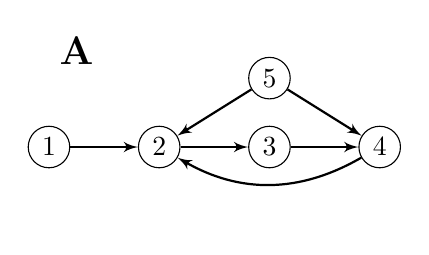
\begin{tikzpicture}[scale=0.7]
					\tikzset{vertex/.style = {shape=circle,draw,minimum 
					size=1.5em, 
							inner 
							sep = 0pt}}
					\tikzset{edge/.style = {->,> = latex', thick}}
					\tikzset{edgebi/.style = {<->,> = latex', thick}}
					\tikzset{every loop/.style={min distance=8mm, looseness=5}}
					\tikzset{vertexFac/.style = {shape=rectangle,draw,minimum 
							size=1.5em, 
							inner sep = 0pt}}
					
					% vertices
					%\draw [line width=35pt,opacity=0.1, blue,line 
					%cap=round,rounded
					%corners] (0,0.5) -- (0,2) -- (-1.5,1.5) -- (0,0.5);
					\node[vertex] (a) at  (-4,0) {$1$};
					\node[vertex] (b) at  (-2,0) {$2$};
					\node[vertex] (c) at  (0,0) {$3$};
					\node[vertex] (d) at  (2,0) {$4$};
					\node[vertex] (e) at  (0,1.25) {$5$};
					
					\node at (-3.5,1.75) {\Large \textbf{A}};
					
					%edges
					
					\draw[edge] (a) to (b);
					\draw[edge] (b) to (c);
					\draw[edge] (c) to (d);
					\draw[edge, bend left = 30] (d) to (b);
					\draw[edge] (e) to (d);
					\draw[edge] (e) to (b);
					\draw[edge, bend right = 35, opacity = 0] (a) to (d);
					
					\end{tikzpicture}
				\end{subfigure}\hspace{.05\linewidth}%
				\begin{subfigure}{0.3\linewidth}
					\centering
					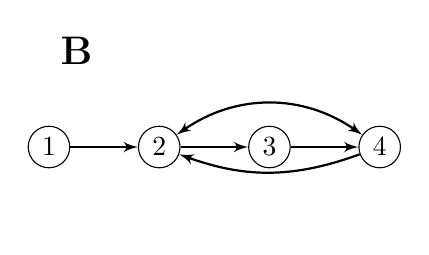
\begin{tikzpicture}[scale=0.7]
					\tikzset{vertex/.style = {shape=circle,draw,minimum 
					size=1.5em, 
							inner 
							sep = 0pt}}
					\tikzset{edge/.style = {->,> = latex', thick}}
					\tikzset{edgebi/.style = {<->,> = latex', thick}}
					\tikzset{every loop/.style={min distance=8mm, looseness=5}}
					\tikzset{vertexFac/.style = {shape=rectangle,draw,minimum 
							size=1.5em, 
							inner sep = 0pt}}
					
					% vertices
					%\draw [line width=35pt,opacity=0.1, blue,line 
					%cap=round,rounded
					%corners] (0,0.5) -- (0,2) -- (-1.5,1.5) -- (0,0.5);
					\node[vertex] (a) at  (-4,0) {$1$};
					\node[vertex] (b) at  (-2,0) {$2$};
					\node[vertex] (c) at  (0,0) {$3$};
					\node[vertex] (d) at  (2,0) {$4$};
					\node[vertex, opacity = 0] (e) at  (0,1.25) {};
					
					\node at (-3.5,1.75) {\Large \textbf{B}};
					
					%edges
					
					\draw[edge] (a) to (b);
					\draw[edge] (b) to (c);
					\draw[edge] (c) to (d);
					\draw[edge, bend left = 20] (d) to (b);
					%\draw[edge] (e) to (d);
					%\draw[edge] (e) to (b);
					\draw[edge, bend right = 35, opacity = 0] (a) to (d);
					\draw[edge, bend left = 35, <->] (b) to (d);
					
					\end{tikzpicture}
				\end{subfigure}\hspace{.05\linewidth}%
				\begin{subfigure}{0.3\linewidth}
					\centering
					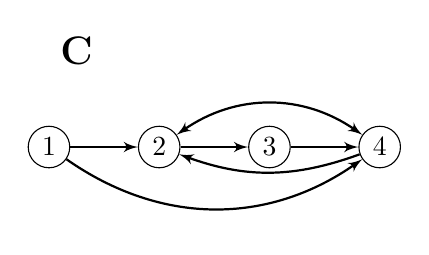
\begin{tikzpicture}[scale=0.7]
					\tikzset{vertex/.style = {shape=circle,draw,minimum 
					size=1.5em, 
							inner 
							sep = 0pt}}
					\tikzset{edge/.style = {->,> = latex', thick}}
					\tikzset{edgebi/.style = {<->,> = latex', thick}}
					\tikzset{every loop/.style={min distance=8mm, looseness=5}}
					\tikzset{vertexFac/.style = {shape=rectangle,draw,minimum 
							size=1.5em, 
							inner sep = 0pt}}
					
					% vertices
					%\draw [line width=35pt,opacity=0.1, blue,line 
					%cap=round,rounded
					%corners] (0,0.5) -- (0,2) -- (-1.5,1.5) -- (0,0.5);
					\node[vertex] (a) at  (-4,0) {$1$};
					\node[vertex] (b) at  (-2,0) {$2$};
					\node[vertex] (c) at  (0,0) {$3$};
					\node[vertex] (d) at  (2,0) {$4$};
					\node[vertex, opacity = 0] (e) at  (0,1.25) {};
					
					\node at (-3.5,1.75) {\Large \textbf{C}};
					
					%edges
					
					\draw[edge] (a) to (b);
					\draw[edge] (b) to (c);
					\draw[edge] (c) to (d);
					\draw[edge, bend left = 20] (d) to (b);
					%\draw[edge] (e) to (d);
					%\draw[edge] (e) to (b);
					\draw[edge, bend right = 35] (a) to (d);
					\draw[edge, bend left = 35, <->] (b) to (d);
					
					\end{tikzpicture}
				\end{subfigure}
				%\end{tabular}
				\caption{\label{fig:smallCycle} \textbf{A}: Directed graph such 
					that 
					each node represents a coordinate process and an edge 
					$\alpha 
					\rightarrow \beta$ implies that $\Phi_{\beta\alpha}\neq 0$. 
					\textbf{B}: Latent projection of the graph \textbf{A} on 
					nodes $O = 
					\{1,2,3,4\}$. \textbf{C}: Graphs \textbf{B} and \textbf{C} 
					are 
					Markov 
					equivalent (entail the same $\mu$-separations), yet are 
					distinguishable using an equality constraint on the 
					observable 
					matrix $\bar{C} = C_{OO}$. Loops 
					(self-edges) are omitted from 
					graphs \textbf{A}, \textbf{B}, and \textbf{C}.}
			\end{figure*}
			
	Consider the graph in Figure \ref{fig:smallCycle}\textbf{A} and assume that 
	this is the causal graph of a Hawkes process on nodes $V = \{1,2,3,4,5\}$ 
	such that coordinate process $5$ is unobserved. Let $\Phi$ be the $4\times 
	4$ matrix of direct effects. If we apply the 
	identification criterion of \cite{weihs2018}, we find that every 
	$\Gamma_{\beta\alpha}$ 
	such that 
	$\alpha,\beta\in O$ is identified from $\Sigma$ (note that 
	$\Gamma_{\beta\alpha}={\Phi}_{\beta\alpha}/(1-{\Phi}_{\beta\beta})$ 
	for $\alpha,\beta\in O$ in this example). It 
	follows 
	from the 
	above propositions that $\Phi_{11}, \Phi_{23}$, and $\Phi_{33}$ are 
	identified from 
	the integrated mean and covariance.
	
	On the other hand, one can show by direct computation that $\Phi_{21}, 
	\Phi_{22}, 
	\Phi_{24}, 
	\Phi_{43},$ and $\Phi_{4,4}$ are not identified. If we consider 
	$\Phi_{21}$, we can 
	understand the lack of identication from the fact that $\Phi_{22}$ 
	cannot 
	be identified. 
	Intuitively, this is explained by its unobserved parent process which 
	implies that we 
	cannot, using only the integrated covariance, separate the contributions 
	from coordinate processes 2 and 5 to the observed covariance. 
\end{exmp}

%%%%%%%%%%%%%%%%%%%%%%%%%%%

\subsection{Identification of cycles}
\label{ssec:idCycles}

The $n$-cycle, $\mathcal{D}_n$, is the directed graph on nodes 
$\alpha_1,\ldots,\alpha_n$ such 
that $\alpha_i \rightarrow \alpha_{i+1}$ for all $i = 1,\ldots,n-1$ and 
$\alpha_n\rightarrow \alpha_1$. When $n \geq 3$, \cite{drton2011} show that 
Equation \ref{eq:covSEM} has at 
most two solutions when the graph is an $n$-cycle and that generically it has 
two solutions. We show in the following that at most one of them is in 
$\mathbb{M}_+^s(\mathcal{G}) \times 
\mathbb{M}_{+,0}^{pd}(\mathcal{G})$, thus, is a solution to the normalized 
Hawkes problem.

\begin{prop}
	Let $\mathcal{G}$ be an $n$-cycle. There is a unique solution 
	to 
	
	$$
	\Sigma = (I - \Gamma)^{-1}\Theta(I - \Gamma)^{-T}
	$$
	
	such that $(\Gamma, \Omega) \in \mathbb{M}_{0,+}^s(\mathcal{G}) \times 
	\mathbb{M}_+^{pd}(\mathcal{G})$.
\end{prop}

\begin{proof}
	Let $(G_0, \Omega_0)$ ,$(G_1, \Omega_1)$ be the two solutions of a linear 
	SEM corresponding to 
	$n$-cycle (generically, they are distinct). We assume that the observed 
	covariance is 
	from a Schur stable system, without loss of generality, say $\rho(G_1) < 
	1$. Let 
	$\delta_i^j$ denote the inverse of the $i$'th diagonal element of 
	$\Omega_j$ and let 
	$\lambda_i^j$ denote the $(i,i+1)$-entry of $G_j$ (modulo $n$). 
	\cite{drton2011} show that,
	
	\begin{align*}
	\delta_i^1 &= \delta_i^0 + \prod_j \delta_j^0 (\prod_j (\lambda_j^0)^2 - 
	1)/\det(K_{-i}) \ \ \ \ \ \ \ \  \text{and} \\
	\delta_i^0 &= \delta_i^1 + \prod_j \delta_j^1 (\prod_j (\lambda_j^1)^2 - 
	1)/\det(K_{-i}),
	\end{align*}
	
	\noindent where $K$ is the inverse of the observed covariance, $\Sigma$, 
	and $K_{-i}$ denotes the submatrix of $K$ with the $i$'th row and column 
	deleted. Replacing $\delta_i^1$ in the lower equation with the expression 
	in the upper equation we obtain, 
	
	\begin{align}
	- (\prod_i \delta_i^1) (\prod_i (\lambda_i^1)^2 - 
	1) = (\prod_i \delta_i^0) (\prod_i (\lambda_i^0)^2 - 
	1).
	\label{eq:deltaLambdaProd}
	\end{align}
	
	\noindent Assume without loss of generality that $\rho(G_0) < 1$, 
	then every eigenvalue of $G_0$ has an absolute value less than 1, and 
	$\det(G_0) < 1$. Due to the structure of $G_0$ it holds that 
	$\det(G_0) = \prod_i(\lambda_i^0)$ such that $\prod_i(\lambda_i^0) < 
	1$ 
	and $\prod_i(\lambda_i^0)^2 < 1$. Every $\delta_i^0$ is 
	positive, and this means that the right-hand side of 
	\ref{eq:deltaLambdaProd} is negative. Every $\delta_i^1$ is positive and 
	therefore we must have $(\prod_i 
	(\lambda_i^1)^2 - 
	1) > 0$ and therefore $(\prod_i 
	(\lambda_i^1) > 1$. This means that $\det(G_1) > 1$ and therefore 
	$\rho(G_1) \geq 1$.
\end{proof}




%%%%%%%%%%%%%%%%%%%%%%%%%%%

\begin{comment}

\subsection{Identifying Link Functions}
\label{ssec:idCauFunc}

It is only natural that we can obtain stronger identification results when we 
use more aspects of the distribution. Following 
\cite{bacry2016}, we define the (non-singular part of) the \emph{infinitesimal 
covariance},

\begin{align}
	v_{\beta\alpha}(t' - t) = E(dN_t^\beta dN_{t'}^\alpha) & - 
	\Lambda^\beta\Lambda^\alpha dt dt' \nonumber \\ & - \Lambda^\beta 
	\varepsilon_{\beta\alpha}
	\delta(t'-t) dt,
	\label{eq:infv}
\end{align}

where $\delta$ is a Dirac delta function and $\varepsilon_{\beta\alpha} = 
\mathds{1}_{(\beta=\alpha)}$, and

$$
g(t) = v^T(t)\Lambda^{-1}.
$$

We let $\Phi(t)$ denote the matrix of functions such that 
$\Phi(t)_{\beta\alpha} = 
\phi_{\beta\alpha}(t)$. \cite{hawkesJRSSB1971} gave the following $n\times n$ 
equality,

\begin{align}
	g(t) = \Phi(t) + \Phi(t) \star g(t),
	\label{eq:covCauFunc}
\end{align}

where $\star$ means that $(\Phi(t) \star g(t))_{\beta\alpha} = \sum_{\gamma \in 
V} 
\int_{-\infty}^{\infty} \phi_{\beta\gamma}(t - s) g_{\gamma\alpha}(s) \md s$. 
\cite{bacry2016} 
prove that if we consider $\Phi(t)$ 
the 
unknown in the above equation, there is a unique solution (such that 
$\phi_{\beta\alpha}$ is in $L^1$ and its support is in $(0,\infty)$ for all 
$\alpha,\beta\in V$).

\begin{prop}
	Let $\mathcal{D} = (O\disjU U, E)$. If $\pa_\mathcal{D}(\beta) \subseteq 
	O$ (that is, all parents of $\beta$ in the causal graph are observed), then 
	for all $\alpha$ the function $\phi_{\beta\alpha}$ is identified 
	from 
	the infinitesimal covariance process of the $O$-processes and 
	$\Lambda_{OO}$.
	\label{prop:gPaId}
\end{prop}

[FIX: this argument does not work]

\begin{proof}
	In Equation \ref{eq:covCauFunc}, we note that $\phi_{\beta\alpha}$ only 
	appears in the $\beta$-row of the equations. Every parent of $\beta$ is 
	observed and therefore this row only depends on observed quantities. If 
	there were two solutions to the equations in the $\beta$-row such that 
	$\phi_{\beta\alpha}$ differed between the two solutions, then there would 
	also 
	be two solutions to Equation (\ref{eq:covCauFunc}) which is a contradiction.
\end{proof}

Under the conditions of Proposition \ref{prop:gPaId}, it also follows 
immediately that $\Phi_{\beta\alpha}$ is identified from the observed 
infinitesimal covariance process and $\Lambda_{OO}$ we will use this in Section 
\ref{ssec:eqInfCov} to obtain further constraints.

\end{comment}

%%%%%%%%%%%%%%%%%%%%%%%%%%%
%%%%%%%%%%%%%%%%%%%%%%%%%%%

\section{Equality Constraints}
\label{sec:eq}

It is well-known that partially observed DAG-models satisfy 
constraints that 
are not described by conditional independence some of which are known as 
\emph{equality constraints}. \cite{richardson2017} treat the general (acyclic) 
case 
while \cite{chen2014, chenNIPS2016} consider equality constraints in linear 
SEMs. In DAG-models equality constraints are testable implications that may 
bring strictly more information about the underlying structure than using 
conditional independence alone. We will see that the analogous statement holds 
for the Hawkes process models, though the relevant notion of independence to 
compare with is 
that of \emph{local independence}. Local independence is an asymmetric notion 
of independence on the coordinate processes of
a multivariate stochastic processes \citep{schweder1970, aalen1987, 
didelez2000, 
didelez2008}. The following definition is specific to point processes, however, 
it can be extended to other classes of stochastic processes 
\citep{aalen1987,didelez2006,mogensenUAI2018,mogensen2018}.

\begin{defn}[Local independence]
	Let $X = (X^1,\ldots,X^n)^T$ be a multivariate point process with intensity 
	processes $\lambda$ and let $V=\{1,\ldots,n\}$. Let $A,B,C,D \subseteq V$. 
	Let $\mathcal{F}_t^D$ denote the natural filtration of $X^D$, i.e., the 
	filtration generated by the coordinate processes in $D$. We say that $X^B$ 
	is \emph{locally independent of $X^A$ given $X^C$} if for all $\beta\in B$ 
	and 
	for all $t\in \mathbb{R}$,
	
	$$
	E(\lambda_t^\beta \mid \mathcal{F}_t^{A\cup C})
	$$
	
	is adapted to the filtration $\mathcal{F}_t^C$.
	\label{def:li}
\end{defn}

Local independence has been used for structure learning in stochastic process 
models 
\citep{meek2014, mogensenUAI2018, thams2019, mogensenUAI2020}, analogously to 
how conditional independence is used for 
constraint-based structure learning in classical models \citep{spirtes1993, 
spirtesSearchChapHandbook}. Structure learning based on local independence 
typically assumes 
\emph{faithfulness}, that is, that $X^B$ is locally independent of $X^A$ given 
$X^C$ if and only if $B$ is $\mu$-separated from $A$ given $C$ in 
$\mathcal{G}$, the DMG 
representing the model
($\mu$-separation, or $\delta$-separation, is a concept analogous to $m$-, or 
$d$-separation \citep{didelez2000, didelez2008, mogensen2018}). The 
\emph{Markov equivalence class} of $\mathcal{G}$ is the set of DMGs that encode 
exactly the same set of $\mu$-separations, 
hence local independences. An obvious 
question is therefore whether there are constraints imposed by the 
 structure that are not described by local independence, or $\mu$-separation. 
 This is indeed the 
 case 
 and such constraints can be used to distinguish between graphical structures 
 that imply the same set of local independences. In the next subsection, we 
 show that one can use the integrated mean and covariance to find such 
 constraints.


\subsection{Using Integrated Covariance}

From Equation \ref{eq:Gtilde} and the section on marginalization we see that 
every equality 
constraint in a linear structural equation model implied by the graphical 
structure imposes the same constraint
on the parameters $(\Gamma, \Theta)$ and this allows us to find 
constraints 
in the Hawkes model. We will show by an example that these constraints may 
provide information about the underlying structure that is not contained the 
Markov equivalence class.

\begin{exmp}
	\label{exmp:eqSmallCycle}
	Consider again the example illustrated by the graph in Figure 
	\ref{fig:smallCycle}\textbf{B}. If we think of the graph as representing a 
	linear SEM, we can, e.g., use Theorem 1 and Lemma 1 of \cite{chen2014} to 
	see that the graphical structure imposes the constraint 
	
	$$\Sigma_{14}/\Sigma_{13} = (\Sigma_{34} - 
	\Gamma_{32}\Sigma_{24})/(\Sigma_{33} - 
	\Gamma_{32}\Sigma_{23}),$$ 
	
	and 
	therefore this algebraic constraint is also satisfied by the Hawkes model 
	corresponding to the graph (note that $\Gamma_{32} = 
	\Phi_{32}/(1-\Phi_{33})$, and that the constraint 
	corresponds to
	two ways of identifying $\Gamma_{43}$). The graphs \textbf{B} and 
	\textbf{C} in Figure 
	\ref{fig:smallCycle} (right) 
	imply the same set of local independences
	when using $\mu$-separation. However, the above constraint is satisfied in 
	\textbf{B} only and therefore this constraint allows us to 
	discriminate between the two models.
\end{exmp}

\begin{comment}


	\begin{figure*}
		%\begin{tabular}{cc}
		\begin{subfigure}{0.3\linewidth}
			\centering
			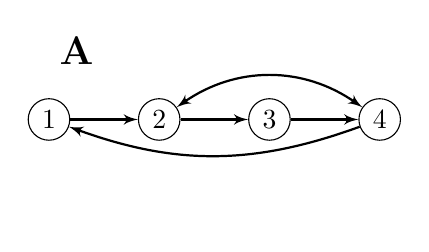
\begin{tikzpicture}[scale=0.7]
			\tikzset{vertex/.style = {shape=circle,draw,minimum size=1.5em, 
					inner 
					sep = 0pt}}
			\tikzset{edge/.style = {->,> = latex', thick}}
			\tikzset{edgebi/.style = {<->,> = latex', thick}}
			\tikzset{every loop/.style={min distance=8mm, looseness=5}}
			\tikzset{vertexFac/.style = {shape=rectangle,draw,minimum 
					size=1.5em, 
					inner sep = 0pt}}
			
			% vertices
			%\draw [line width=35pt,opacity=0.1, blue,line cap=round,rounded
			%corners] (0,0.5) -- (0,2) -- (-1.5,1.5) -- (0,0.5);
			\node[vertex] (a) at  (-4,0) {$1$};
			\node[vertex] (b) at  (-2,0) {$2$};
			\node[vertex] (c) at  (0,0) {$3$};
			\node[vertex] (d) at  (2,0) {$4$};
			\node[vertex, opacity = 0] (f) at  (-1,-1.5) {};
			
			\node at (-3.5,1.25) {\Large \textbf{A}};
			
			%edges
			
			\draw[edge] (a) to (b);
			\draw[edge] (b) to (c);
			\draw[edge] (c) to (d);
			\draw[edge, bend left = 20] (d) to (a);
			
			
			\draw[edge, bend left = 35, <->] (b) to (d);			
			
			
			
			\end{tikzpicture}
		\end{subfigure}\hspace{0.05\linewidth}%
		\begin{subfigure}{0.3\linewidth}
			\centering
			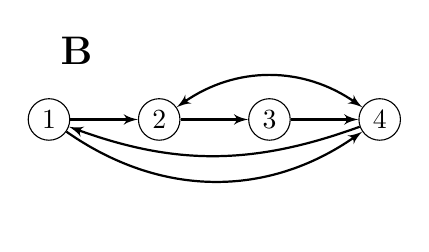
\begin{tikzpicture}[scale=0.7]
			\tikzset{vertex/.style = {shape=circle,draw,minimum size=1.5em, 
					inner 
					sep = 0pt}}
			\tikzset{edge/.style = {->,> = latex', thick}}
			\tikzset{edgebi/.style = {<->,> = latex', thick}}
			\tikzset{every loop/.style={min distance=8mm, looseness=5}}
			\tikzset{vertexFac/.style = {shape=rectangle,draw,minimum 
					size=1.5em, 
					inner sep = 0pt}}
			
			% vertices
			%\draw [line width=35pt,opacity=0.1, blue,line cap=round,rounded
			%corners] (0,0.5) -- (0,2) -- (-1.5,1.5) -- (0,0.5);
			\node[vertex] (a) at  (-4,0) {$1$};
			\node[vertex] (b) at  (-2,0) {$2$};
			\node[vertex] (c) at  (0,0) {$3$};
			\node[vertex] (d) at  (2,0) {$4$};
			\node[vertex, opacity = 0] (f) at  (-1,-1.5) {};
			
			\node at (-3.5,1.25) {\Large \textbf{B}};
			
			%edges
			
			\draw[edge] (a) to (b);
			\draw[edge] (b) to (c);
			\draw[edge] (c) to (d);
			\draw[edge, bend left = 20] (d) to (a);
			\draw[edge, bend right = 35] (a) to (d);			
			
			\draw[edge, bend left = 35, <->] (b) to (d);			
			
			
			
			\end{tikzpicture}
		\end{subfigure}\hspace{0.05\linewidth}%
		\begin{subfigure}{0.3\linewidth}
			\centering
			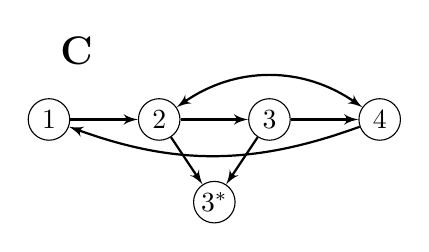
\begin{tikzpicture}[scale=0.7]
			\tikzset{vertex/.style = {shape=circle,draw,minimum size=1.5em, 
					inner 
					sep = 0pt}}
			\tikzset{edge/.style = {->,> = latex', thick}}
			\tikzset{edgebi/.style = {<->,> = latex', thick}}
			\tikzset{every loop/.style={min distance=8mm, looseness=5}}
			\tikzset{vertexFac/.style = {shape=rectangle,draw,minimum 
					size=1.5em, 
					inner sep = 0pt}}
			
			% vertices
			%\draw [line width=35pt,opacity=0.1, blue,line cap=round,rounded
			%corners] (0,0.5) -- (0,2) -- (-1.5,1.5) -- (0,0.5);
			\node[vertex] (a) at  (-4,0) {$1$};
			\node[vertex] (b) at  (-2,0) {$2$};
			\node[vertex] (c) at  (0,0) {$3$};
			\node[vertex] (d) at  (2,0) {$4$};
			\node[vertex] (f) at  (-1,-1.5) {$3^*$};
			
			\node at (-3.5,1.25) {\Large \textbf{C}};
			
			%edges
			
			\draw[edge] (a) to (b);
			\draw[edge] (b) to (c);
			\draw[edge] (c) to (d);
			\draw[edge, bend left = 20] (d) to (a);
			\draw[edge] (b) to (f);
			\draw[edge] (c) to (f);
			
			\draw[edge, bend left = 35, <->] (b) to (d);			
			
			\end{tikzpicture}
		\end{subfigure}
		%\end{tabular}
		\caption{\label{fig:bigCycle} Graphs \textbf{A} and \textbf{B} are 
			Markov equivalent, that is, entail the same local independences 
			(assuming faithfulness). They can be distinguished using an 
			equality constraint arising from using dynamical information as 
			well 
			(see Example \ref{exmp:eqBigCycle}). Graph \textbf{C} illustrates 
			the 
			use of an \emph{auxiliary variable}, see Example 
			\ref{exmp:eqBigCycle}.
			Loops (self-edges) 
			are omitted from this 
			vizualiation.}
	\end{figure*}
	
\end{comment}


\begin{comment}


\subsection{Using Infinitesimal Covariance}
\label{ssec:eqInfCov}

The above subsection describes constraints that are imposed by the graphical 
structure on the integrated 
covariance. If we use other aspects of 
the distribution, 
we can obtain more constraints. In this subsection, we use Proposition 
\ref{prop:gPaId} to identify some of the entries in $\Phi$. We then treat these 
parameters as known in the integrated covariance equation which allows us to 
obtain more constraints. This is similar to previous work on identification in 
linear structural equations models with prior knowledge  
\citep{chenIJCAI2016,chenICML2017}.

\begin{exmp}
	
	
	We consider graph \textbf{A} in Figure \ref{fig:bigCycle}. The constraint 
	from Example \ref{exmp:eqSmallCycle} does not hold in this graph. Instead 
	we assume in 
	this example that we also have access to the 
	covariance processes. In this case, the link functions 
	$\phi_{11},\phi_{14},\phi_{32}$, and $\phi_{33}$ are identified 
	(Proposition 
	\ref{prop:gPaId}), and therefore so are $\Phi_{11}, \Phi_{14} , \Phi_{32}$ 
	and 
	$\Phi_{33}$.  Leveraging this information we can again find two ways of 
	identifying 
	$\Gamma_{43}$ and from this we will obtain an equality constraint 
	that 
	will 
	discriminate between graphs \textbf{A} and \textbf{B} in 
	Figure \ref{fig:bigCycle}. This can be done in different ways. We 
	construct an {\it auxiliary 
	variable} following \cite{chenIJCAI2016, chenICML2017}. This can be thought 
	of as a technique to leverage known coefficients to obtain additional 
	identification or constraints for a given model. Let $O=\{1,2,3,4\}$ and 
	let $\Phi^+$ be a 
	$5\times 5$ 
	matrix such that $\Phi_{OO}^+ = \Gamma$, $\Phi_{52}^+ = 
	-\Gamma_{32}, \Phi_{53}^+ 
	= 1$, and else zero, and we let $\Theta^+$ be a $5\times 5$ matrix such 
	that $\Theta_{OO}^+ = \Theta$, and $\Theta_{55}^+ = 1$ and zero else. This 
	construction corresponds to a linear SEM where we added an \emph{auxiliary 
	variable}, $3^*$, to the original model, see \ref{fig:bigCycle}\textbf{C}. 
	Then 
	the matrix $C^+$,
	
	$$
	C^+ = (I - \Phi^+)^{-1}\Theta^+(I-\Phi^+)^{-1},
	$$
	
	can be computed from $\bar{C}$ and it holds that 
	$C^+=\bar{C}_{OO}$. By direct computation, we see that $\Gamma_{43} = 
	C_{14}^+/C_{13}^+$. To obtain a constraint, we find a second method of 
	identification of $\Gamma_{43}$ by noting that
	
	\begin{align}
		\Theta = (I - \Gamma)\bar{C}(I-\Gamma)^T = \bar{C} - 
		\Gamma\bar{C} - \bar{C}\Gamma^T + 
		\Gamma\bar{C}\Gamma^T,
		\label{eq:expandTheta}
	\end{align}

	
	assuming that $\Gamma$ is weakly stable. By considering the 
	$(3,4)$-entry of the above matrix equation,
	
	$$
	\Gamma_{43} = (\bar{C}_{34} - 
	\Gamma_{32}\bar{C}_{24})/(\bar{C}_{33} - 
	\Gamma_{32}\bar{C}_{23}).
	$$
	
 Again, we obtained two ways of identifying 
 the parameter $\Gamma_{43}$, that is, a constraint
 
 $$
 C_{14}^+/C_{13}^+ = (\bar{C}_{34} - 
 \Gamma_{32}\bar{C}_{24})/(\bar{C}_{33} - 
 \Gamma_{32}\bar{C}_{23})
 $$
 
 using that $\Gamma_{32} = {\Phi}_{32}/(1-\Phi_{33})$ is known as 
 ${\Phi}_{32}$ and 
 ${\Phi}_{33}$ are known. This constraint is satisfied in 
 Figure
 \ref{fig:bigCycle}\textbf{A}, 
 but not in \ref{fig:bigCycle}\textbf{B}, and it allows us to 
 distinguish between 
 the two.
 
 \label{exmp:eqBigCycle}
\end{exmp}


\end{comment}


%%%%%%%%%%%%%%%%%%%%%%%%%%%
%%%%%%%%%%%%%%%%%%%%%%%%%%%

\section{Ideas/Notes}

FIX: stress throughout that the central idea is to use something 
time-independent to find equality constraints

check everything, also numerically - check also n-cycle proof, different 
formula for delta is used (there seems to be an error in Drton2011)

Formulate more clearly that id in SEMs relate to the marginalized and 
normalized Hawkes problem!

In n-cycle example: Note that if $G_0$, $G_1$ are the 
two solutions, then it holds that $det(G_0)det(G_1) = 1$, use this to prove 
this? (both solutions will have positive entries only). Note also that for a 
linear SEM Graph A in \ref{fig:bigCycle} generically has only two solutions - 
just like the 4-cycle. Can I show that only one satisfies spectral constraint 
(using the conjecture from above that this is implied by the spectral 
constraint in the full system)



Note that for positive matrices, it seems that spectral radius less than one in 
the full system entails spectral radius less than one in the marginal system 
(tested empirically) (interlacing property of Schur complements?) - contrary to 
lin SEMs system, and what I write earlier in this paper.



Question: find an example where one does not have generic ID with these 
additional constraints. check that one does not have generic id for all graphs!

Re-write to define an actual Hawkes covariance model? Define parameter space 
etc, makes it clear what id is, and what the problems amount to - also in 
comparison with lin SEM work.

\section{Conclusion}

We obtained identification results and equality constraints for Hawkes process 
models through the similarity between integrated Hawkes covariance and observed 
covariance of a linear structural equation model. These 
equality constraints are useful for structure learning as they can 
supplement constraint-based learning based on tests of local independence. The 
approach in this paper finds equality constraints through a time-independent 
statistic which may be applicable in other classes of stochastic processes as 
well.

A Hawkes process is defined using the set of $\phi_{\beta\alpha}$-functions 
along 
with the $\mu_\alpha$-constants for $\alpha,\beta$ in the finite set $V$ and a 
Hawkes process model is in that sense nonparametric.  Constraints that arise 
from the integrated covariance offer also a dimension reduction in that we  
test these constraints using a finite parameter space instead of a 
function space. This makes them more suitable to employ in data analysis 
as estimation of the link functions, $\{\phi_{\beta\alpha} \}$, is a 
challenging problem even in the case of full 
observation and partial observation only adds to the 
complexity of this task.



%%%%%%%%%%%%%%%%%%%%%%%%%%%
%%%%%%%%%%%%%%%%%%%%%%%%%%%


\begin{contributions} % will be removed in pdf for initial submission,
                      % so you can already fill it to test with the
                      % ‘accepted’ class option

\end{contributions}

\begin{acknowledgements} % will be removed in pdf for initial submission,
                         % so you can already fill it to test with the
                         % ‘accepted’ class option
    This work was supported by a research grant from
    VILLUM FONDEN (13358) and by a DFF-International Postdoctoral Grant 
    (0164-00023B) from Independent Research Fund Denmark.
\end{acknowledgements}

\appendix

\section{Marginalization}
\label{sec:marg}

In this section and for a matrix $A$, we define $A_{\bar{I}\bar{J}}^{-1} = 
(A^{-1})_{\bar{I}\bar{J}}$ and 
$A_{\bar{I}\bar{J}}^{-T}=(A^{-T})_{\bar{I}\bar{J}}$. Consider an invertible 
block matrix 

$$
M=
\begin{pmatrix}
A & B \\
C & D
\end{pmatrix}.
$$

We let $M / D = A - BD^{-1}C$ denote the \emph{Schur complement} of block D in 
the matrix M. It holds that

$$
M^{-1}=
\begin{pmatrix}
(M/D)^{-1} & -(M/D)^{-1}BD^{-1} \\
-D^{-1}C(M/D)^{-1} & D^{-1}(I + C(M/D)^{-1}BD^{-1})
\end{pmatrix}.
$$

Therefore, $$(I - {\Phi})_{OO}^{-1} = ((I - {\Phi})/(I - 
{\Phi})_{UU})^{-1} = (I- \bar{\Phi})^{-1}$$ by definition of 
$\bar{\Phi}$. 
Furthermore, 

$$
(I-{\Phi})_{OU}^{-1} = 
-(I-\bar{\Phi})^{-1}(I-{\Phi})_{OU}(I-{\Phi})((I-{\Phi})_{UU})^{-1}
$$

Let $I = I_n$ and $A_{\bar{I}}=A_{\bar{I}\bar{I}}$. From the above, it 
follows 
that

\begin{align*}
\Theta & = (I_k - \bar{\Phi})[(I_n - 
{\Phi})_{O}^{-1}{\Lambda}_{O}(I - {\Phi})_{O}^{-T} + \\ 
&  
(I 
- 
{\Phi}_{OU}^{-1}){\Lambda}_{U}(I - 
{\Phi})_{UO}^{-T}](I_k - 
\bar{\Phi})^T \\
& = {\Lambda}_{O} + (I_k - \bar{\Phi})(I 
- 
{\Phi})_{OU}^{-1}{\Lambda}_{U}((I - 
{\Phi})_{UO}^{-T}(I_k - 
\bar{\Phi})^T \\
& = {\Lambda}_{O} + \\ & (I - {\Phi})_{OU}(I - 
{\Phi})_{U}^{-1}{\Lambda}_{U}((I - 
{\Phi})_{U}^{-T}(I - 
{\Phi})_{U}^{-T}(I - 
{\Phi})_{OU}^T \\
& = {\Lambda}_{O} + {\Phi}_{OU}(I - 
{\Phi})_{U}^{-1}{\Lambda}_{U}((I - 
{\Phi})^{-T})_{U}(I - 
{\Phi})_{U}^{-T} 
{\Phi}_{OU}^T \\
& = {\Lambda}_{O} + {\Phi}_{OU}(I - 
{\Phi})_{U}^{-1}{\Lambda}_{U} (I - 
{\Phi})_{U}^{-T}
{\Phi}_{OU}^T.
\end{align*}


\bibliography{parentalLearning,C:/Users/swmo/Desktop/-/UCPH/PhD/learning/parental/causalScreening/parentalLearning}
\end{document}
